FM-indeks je samostojeći indeks koji su 2000. godine u svom radu opisali i objavili Ferragina i Manzini \cite{fm1}. Općenito indeks je podatkovna struktura koja omogućuje učinkovito dohvaćanje podataka. Samostojeći indeks (engl. \emph{self-index}) je struktura koja se stvara nad određenim tekstom te ga indeksira na način da je memorijski proporcionalna veličini komprimiranog teksta te omogućava efikasno dohvaćanje i prebrojavanje dijelova tog teksta (bez potrebe za dekompresijom cijelog teksta).
Osim originalne implementacije opisane u nastavku, tokom godina napravljene su različite inačice FM-indeksa (npr. \emph{Alphabet-Friendly FM-index} - Ferragina, 2004.).

\section{Originalna implementacija}
FM-indeks count je implementacija FM-indeksa koja služi za pronalaženje broja pojavljivanja uzorka P u tekstu S. Općenito se FM-indeks temelji na Burrows-Wheeler transformaciji i sufisknom polju, ali kod izvedbe samo prebrojavanja, ne i dohvaćanja svih pojavljivanja (FM-indeks find), struktura sufiksnog polja se može izostaviti.
FM-indeks count je ustvari samo izvedba algoritma pretraživanja unatrag  (engl. \emph{backward search}) u kojemu se kreće s pretraživanjem od zadnjeg znaka uzorka P te ako uzorak postoji u tekstu, algoritam vraća koliko se puta on u tekstu ponavlja.
Pronalaženje broja pojavljivanja uzorka u tekstu provodi se tako da se nad zadanim tekstom prvo stvori FM-indeks sa svojim strukturama OCC tablicom i C tablicom te se zatim koristeći stvorene tablice provodi prebrojavanje za zadani uzorak.
U originalnoj implementaciji FM-indeksa, algoritam pretraživanja unatrag se provodi nad nizom znakova koji je dobiven iz originalnog teksta na koji su primijenjene različite operacije \cite{fm1}. Nad originalnim tekstom provedene su redom Burrows-Wheeler transformacija, \emph{Move-To-Front} i \emph{Run-length} kodiranje te stvaranje prefiksnog koda promjenjive duljine.  Za provođenje algoritma potrebne su funkcije C(c) i Occ(c,i). C(c) daje broj znakova u (originalnom) tekstu koji su abecedno prije znaka c uključujući i ponavljanje pojedinih znakova. Occ(c,i) daje broj pojavljivanja znaka c u nizu B[1,i], i=1...$|S|$, gdje je S originalni tekst, B niz dobiven transformacijama originalnog teksta, a znak c je bilo koji znak iz abecede originalnog teksta. Pokazano je da brzina izvođenja funkcije Occ(c,i) određuje brzinu izvođenja cijelog algoritma pretraživanja unatrag \cite{fm2}. U originalnoj implementaciji funkcija Occ(c,i) se računa korištenjem transformiranog (sažetog) originalnog teksta te nekoliko dodatnih pomoćnih struktura. 



\section{Implementacija FM-indeksa}
U ovoj implementaciji FM-indeksa koristi se algoritam pretraživanja unatrag i ranije spomenuta struktura C tablice na isti način kao i u originalnoj implementaciji, ali je funkcija Occ(c,i) izvedena korištenjem wavelet stabla i RRR struktura čiji je princip objašnjen u ranijem poglavlju, a napravljen po uzoru na \cite{fm3}.

Prvi korak je dodavanje znaka \$ na kraj niza te stvaranje C tablice koja za svaki znak iz abecede ulaznog teksta sadrži informacije koliko je znakova abecedno manjih ispred tog znaka abecede, uključujući i ponavljanje znakova. Pretpostavimo da ulazni niz s nadodanim znakom kraja niza glasi \emph{ACAAGATGCACAATGTCCCA\$}. Stvorena struktura (C tablica) izgledala bi ovako:

\begin{table}[htb]
\caption{C tablica}
\label{tbl:ctabl}
\centering
\begin{tabular}{|l||ccccc|} \hline
c & \$ & A & C & G & T \\ \hline
C(c) & 0 & 1 & 9 & 15 & 18 \\ \hline
\end{tabular}
\end{table}

\vspace{3 mm}
Sljedeći korak je provođenje Burrows-Wheeler transformacije nad zadanim tekstom  \linebreak korištenjem sufiksnog polja, čime se iz niza \emph{ACAAGATGCCAATGTCCCA\$} dobiva niz \emph{ACCC\$CAGACAAGCTATTGAA}. BWT i algoritam izgradnje sufiksnog polja detaljno su opisani u prethodnom poglavlju.
Na temelju dobivenog niza stvara se OCC tablica koja je u ovoj implementaciji predstavljena wavelet stablom. Na temelju izgrađenog stabla prikazanog slikom  \ref{fmWaveletTree}, uz korištenje RRR struktura koje se stvaraju za svaki list stabla (i služe za računanje broja jedinica u dijelu niza pojedinog lista), lako se računaju  vrijednosti Occ(c,i) koje su potrebne za algoritam pretraživanja unatrag. Struktura wavelet stabla i RRR struktura su detaljnije opisane u ranijim potpoglavljima. 


\begin{figure}[H]
\centering
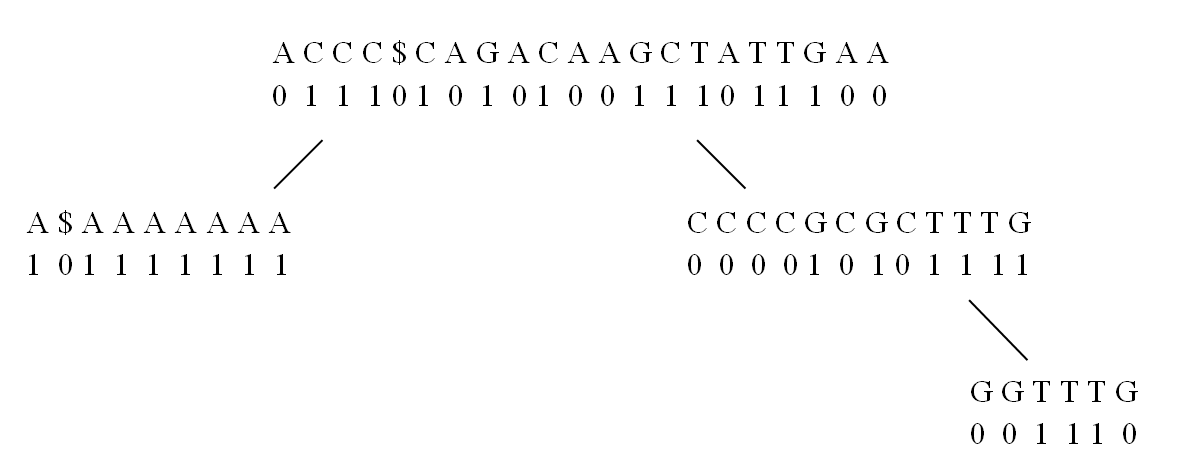
\includegraphics[width=\linewidth]{./pictures/fmStablo.png}
\caption{Prikaz izgrađenog wavelet stabla za niz \emph{ACCC\$CAGACAAGCTATTGAA}}\label{fmWaveletTree}
\end{figure}

Ovim dijelom implementacije završeno je stvaranje same strukture FM-indeksa te je još samo potrebno implementirati algoritam koji će obuhvatiti prebrojavanje pojavljivanja nekog podniza u nizu nad kojim je napravljen FM-indeks, tj. \emph{Count} dio implementacije indeksa.

Za završni dio implementacije korišten je algoritam pretraživanja unatrag (engl. \emph{backward search algorithm}). Algoritam je implementiran kao i u originalnoj implementaciji FM-indeksa \cite{fm1}, prema sljedećem pseudokodu:


\begin{algorithm}
\caption{ Pretraživanje unatrag }
\label{algo:bws}
\begin{algorithmic}
\STATE{\textbf{Ulaz:} P[0, p - 1] -- zadani podniz}
\STATE{\textbf{Izlaz:} broj pojavljivanja podniza}
\STATE{i = p - 1;}
\STATE{c = P[i];}
\STATE{startPosition = C[c] + 1;}
\STATE{endPosition = C[c + 1];}
\FOR{(i=i-1; i$>=$0; i-\--)}
\STATE{c = P[i];}
\STATE{startPosition = C[c] + Occ(c, startPosition - 2) + 1;}
\STATE{endPosition = C[c] + Occ(c, endPosition - 1);}
\ENDFOR
\IF{endPosition $>=$ startPosition}
\RETURN endPosition - startPosition + 1;
\ELSE
\RETURN 0;
\ENDIF
\end{algorithmic}
\end{algorithm}


\vspace{3 mm}

Ako se i dalje pretpostavi da se FM-indeks izgradio nad nizom \emph{ACAAGATGCCAATGTCCCA}  u kojemu se želi pronaći broj pojavljivanja podniza \emph{ATG}, algoritam pretraživanja unatrag se provodi prema sljedećim koracima:

\vspace{2 mm}

\textbf{Inicijalizacija:} \newline
i = 2; \newline
c = 'G'; \newline
startPosition = 15 + 1 = 16; \newline
endPosition = 18; \newline
\newline
\textbf{1. korak petlje:} \newline
i = 1; \newline
c = 'T'; \newline
startPosition  = 18 + 1 + 1 = 20; \newline
endPosition = 18 + 3 = 21; \newline
\newline
\textbf{2. korak petlje:} \newline
i = 0; \newline
c = 'A'; \newline
startPosition  = 1 + 6 + 1 = 8; \newline
endPosition = 1 + 8 = 9; \newline
PETLJA STOP \newline
 \newline
\textbf{Izlaz:} broj pojavljivanja = 9 - 8 + 1 = \textbf{2} 


\section{Nedostaci implementacije u programskom jeziku Java}
Implementacija ovog algoritma napravljena je u programskom jeziku Java.  Iako Java kao programski jezik nudi mnoge pogodnosti, kao jednostavnu sintaksu, dobre popratne biblioteke i automatsko upravljanje memorijom, ipak postoje i određeni nedostatci ovakvog jezika. Možda najveći nedostatak Java programskog jezika dolazi upravo od jedne predosti samog jezika, a to je automatsko upravljanje memorijom. To znači da se programski jezik sam brine oko oslobađanja i zauzimanja memorije, što može biti problematično prilikom izvođenja aplikacije koje troše puno memorije. U tim slučajevima potrebno je ručno pozvati \textit{garbage collector} kako bi oslobodio zauzetu memoriju, no to nažalost opet ima utjecaj na brzinu izvođenja, posebno ukoliko je takvih poziva više. Osim toga, Java virtualni stroj često zauzme više memorije nego joj je uistinu potrebno, što se jako dobro može vidjeti korištenjem alata za profiliranje. To svakako predstavlja problem ukoliko program prilikom izvođenja zauzima velike količine memorije, jer se one dodatno povećaju zbog tog praznog prostora kojeg zauzme Java virtualni stroj. Iako postoje naredbe kojima se može pokušati regulirati količina memorije koju će virtualna stroj smjeti zauzeti, kao i naredbe kojima bi se trebalo moći natjerati virtualnu stroj da memoriju koju je zauzela, a ne koristi ju, vrati operacijskom sustavu, uočeno je kako je potrebno dobro podesiti parametre tih naredbi prilikom izvođenja kako bi se dobili što bolji rezultati. Osim toga, Java virtualni stroj sam po sebi zauzima dosta veliku količinu memorije (prilikom testiranja to je otprilike bilo oko 10MB), što svakako predstavlja još jedan nedostatak programskog jezika Java. Možda se memorija od 10MB ne čini kako velika količina memorije, posebice uzevši u obzir raspoloživu količinu memorije u današnjim računalima, no svejedno nije to ni zanemariva količina memorije, posebice ako se indeksiraju kraći znakovni nizovi.

Još jedan nedostatak Java programskog jezika jest što primitivni tip podatka \textit{char} zauzima dva bajta memorije. To znači da zapravo imamo dvostruko veću memorijsku složenost nego što bi htjeli. Iz tog razloga, u implementaciji se koristi tip podatka \textit{byte} kako bi se uštedjelo na memoriji. Time je limitiran broj različitih znakova koje možemo prikazati, no kako je glavni fokus ipak stavljen na DNA sekvence i nizove proteina, ovo ograničenje ne predstavlja veliki problem. Dodatno je postavljeno još jedno ograničenje, a to je da implementacija može raditi nad osnovnim skupom \textit{ASCII} znakova. To je napravljeno iz razloga što Java programski jezik nema \text{unsigned} inačice tipova podataka (opet jedan veliki nedostatak), te ukoliko bi se htjelo raditi nad proširenim skupom \textit{ASCII} znakova, moralo bi se paziti na preslikavanje negativnih vrijednosti u njihove pozitivne ekvivalente, zadržavajući leksički poredak. Taj postupak bi uveo dodatne operacije koje bi mogle utjecati na performanse izvođenja ovog algoritma, te iz tog razloga nije napravljen (iako doduše implementaciju nije teško proširiti tako da radi i s proširenim skupom \textit{ASCII} znakova). 

Konačno, upitna je i brzina Java programskog jezika naspram jezika C/C++. Ovdje se neće ulaziti u detalje oko tog pitanja, jer različiti izvori nude različita mjerenja performansi. Programi koji su napisani u programskom jeziku Java obično postižu nešto lošije rezultate, no to sve ovisi o tome koliko su efikasno napravljene pojedine implementacije, kao i o problemu koji je rješavan. 



